\documentclass[11pt]{article}
\usepackage[catalan]{babel}
\usepackage{graphicx}
\usepackage[margin=1in]{geometry}
\usepackage{fancyhdr}
\usepackage{lipsum}
\usepackage{amsmath}
\usepackage{tikz-uml}
\tikzumlset{fill usecase=white}
\usepackage[hidelinks]{hyperref}
\pagestyle{fancy}

\title{\bfseries\Huge OrionWay}
\author{RLP - Grup 5}

\rhead{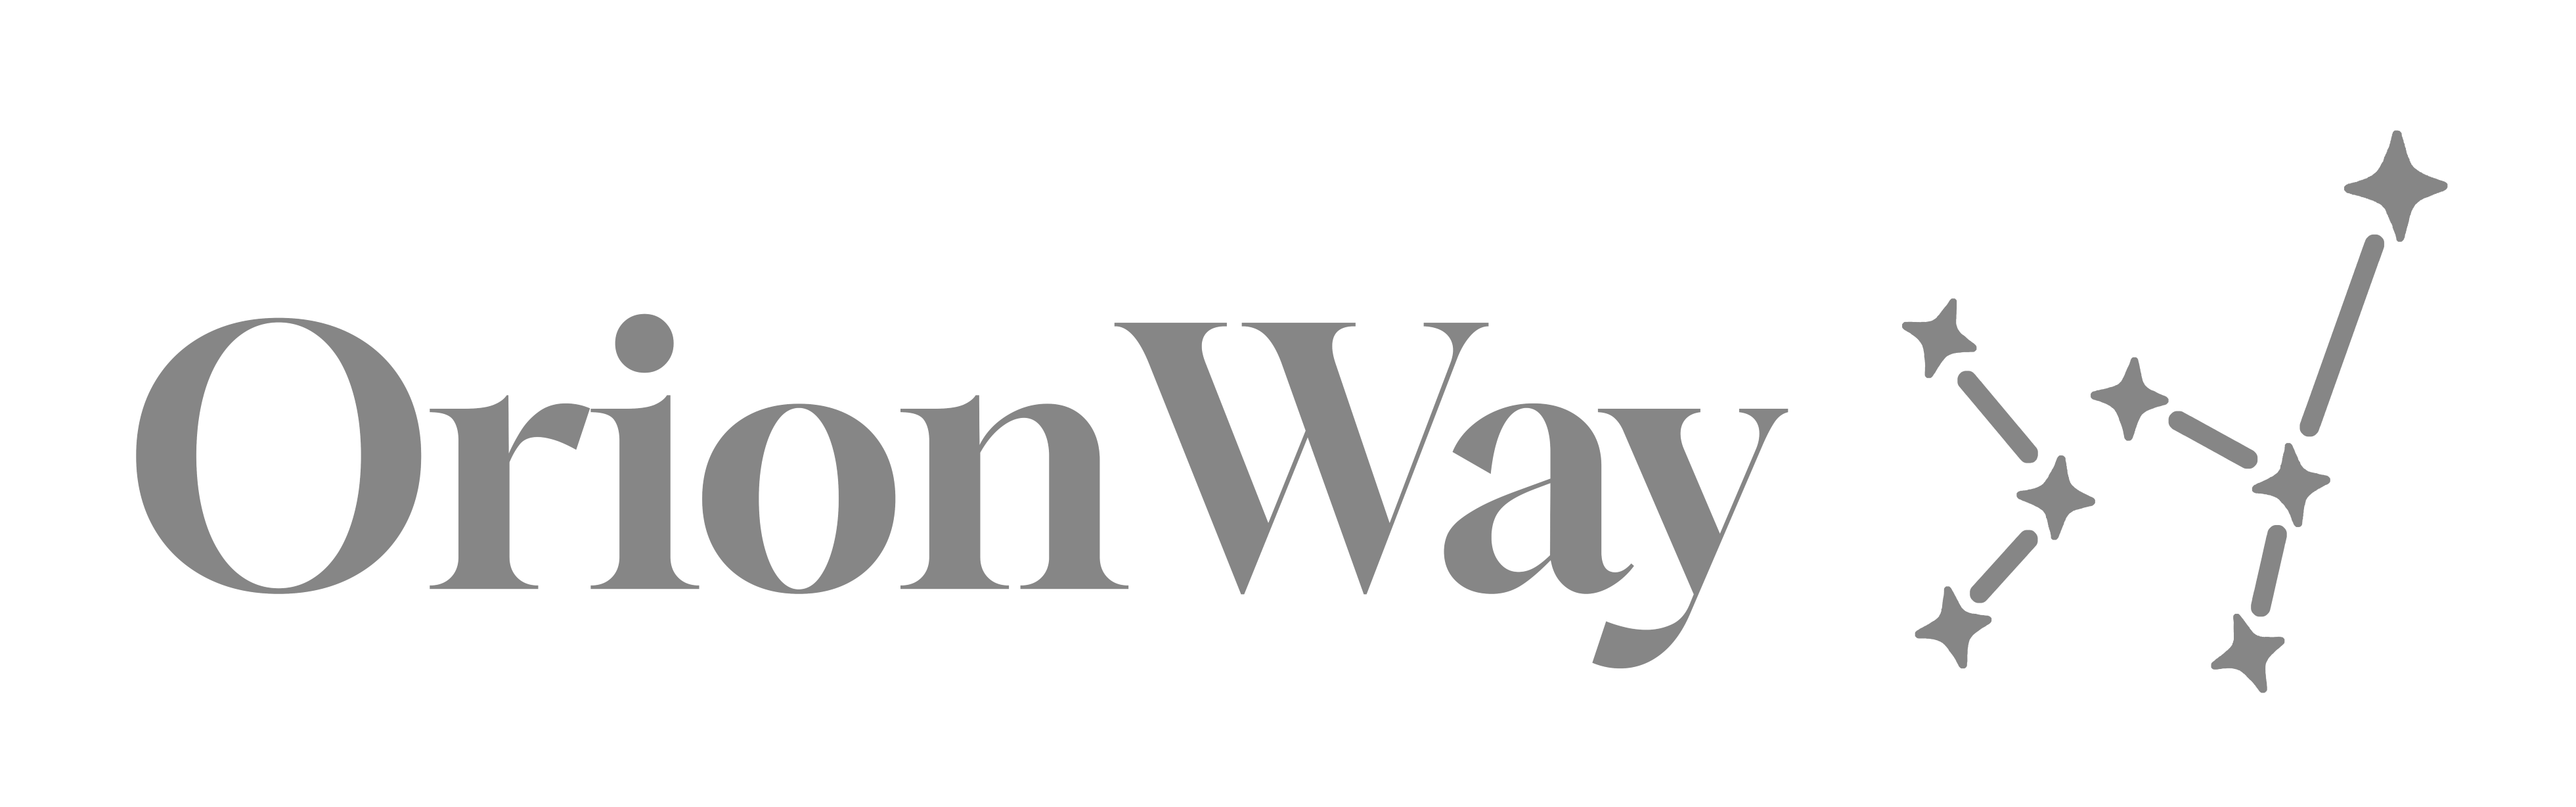
\includegraphics[height=0.08\linewidth]{../orionway_transparent}}
\renewcommand{\headrulewidth}{0pt}
\renewcommand{\footrulewidth}{0pt}
\setlength{\headsep}{1.5cm}

\usetikzlibrary{positioning,fit,arrows.meta,backgrounds}
\tikzset{
	module/.style={
		draw,
		minimum width=#1,
		minimum height=7mm,
		align=center
	},
	module/.default=2cm,
	>=LaTeX
}

\begin{document}
	
	%\maketitle
	%\begin{abstract}
	%\end{abstract}
	%\newpage
	\begin{center}
		\vspace*{0.25cm}
		{\Huge \bfseries Diagrames de Software}\\[0.5cm]
		{\Large RLP - Grup 5}\\[0.25cm]
		\today
	\end{center}
	
	\section*{Diagrama de casos d'ús}
	
	 \begin{tikzpicture}
		\begin{umlsystem}[x=4, draw=none] {} 
			\umlusecase[name=x,x=4,y=2.5,width=2cm] {Reconeixement d'objectes}
			\umlusecase[name=a,x=4,y=00.5,width=2cm] {Aturar robot}
			\umlusecase[name=b,x=0.1,y=-2,width=2cm] {Control manual}
			\umlusecase[name=c,x=4,y=-2,width=2cm] {Revisar obstacles}
			\umlusecase[name=d,x=8,y=-2,width=2.5cm] {Revisar passos de zebra}
			\umlusecase[name=e,x=4,y=-6,width=2cm] {Navegació}
			\umlusecase[name=f,x=4,y=-8,width=2cm] {Apropament automàtic}
		\end{umlsystem}
		
		\umlactor[y=0] {Botons}
		\umlactor[x=15, y=-5] {Ultrasons}
		\umlactor[x=15, y=0] {Càmera}
		\umlactor[x=15, y=2.5] {Altaveu}
		\umlactor[y=-6] {Micròfon}
		
		\umlassoc{Botons}{a}
		\umlassoc{Botons}{b}
		\umlassoc{Botons}{x}
		\umlassoc{Ultrasons}{c}
		\umlassoc{Càmera}{x}
		\umlassoc{Càmera}{d}
		\umlassoc{Altaveu}{x}
		\umlassoc{Micròfon}{f}
		
		
		\draw [tikzuml dependency style] (f) -- node[pos=0.5] {$\ll \text{extend} \gg$} (e);
		\draw [tikzuml dependency style] (e) -- node[pos=0.4] {$\ll \text{include} \gg$} (c);
		\draw [tikzuml dependency style] (e) -- node[pos=0.6] {$\ll \text{include} \gg$} (b);
		\draw [tikzuml dependency style] (e) -- node[pos=0.6] {$\ll \text{include} \gg$} (d);
		\draw [tikzuml dependency style] (c) -- node[pos=0.5] {$\ll \text{include} \gg$} (a);
		\draw [tikzuml dependency style] (d) -- node[pos=0.3] {$\ll \text{include} \gg$} (a);

		\draw [tikzuml association style] (e) to[bend left=22] (Botons);
		\draw [tikzuml association style] (f) to[bend right=25] (Càmera);
	\end{tikzpicture}
	\section*{Diagrama de mòduls}
%		\begin{tikzpicture}
%				
%		% Place first 6 items
%		\node[module] (I3) {\texttt{DetectorBotons}};
%		\node[module=1cm, below=8mm of I3] (I5) {Item-5};
%		\node[module=1cm, left= 3mm of I5] (I4) {Item-4};
%		\node[module=1cm, right= 3mm of I5] (I6) {Item-6};
%		\node[module, below=of I5] (I2) {Item-2};
%		\node[module, below=of I2] (I1) {Item-1};
%		
%		
%		% Inner box around Items 3-6 with rounded corners
%		\node[label={\textbf{Sensors}}, fit=(I3) (I4) (I6), draw, inner sep=2mm, rounded corners] (sensors) {};
%		
%		% Outer box around all left items with rounded corners
%		\node[fit=(sensors) (I1), draw, inner sep=2mm, inner ysep=8mm, rounded corners] (fit1) {};
%		\node[anchor=south] at (fit1.north) {\textbf{Vistes}};
%		
%		% Connections
%%		\foreach \i in {4,5,6}
%%		\draw[->] (I3)--(I\i);
%%		\draw[->] (I2)--(I1);
%%		\draw[->] (I2)--(sensors);
%		
%		% Items 7-8-9. Item 7 as label of Item-8
%		\node[module, right=2cm of {I2-|fit1.east}, 
%		label={[yshift=5mm, font=\rmfamily]Item-7}] 
%		(I8) {Item-8};
%		\node[module, below=of I8] (I9) {Item-9};
%		
%		% Outer box around items 8-9 with rounded corners
%		\node[fit={(I9) (I9|-fit1.south) (I9|-fit1.north)}, draw, inner xsep=5mm, inner ysep=-\pgflinewidth, rounded corners] (fit8) {};
%		
%		\node[anchor=south] at (fit8.north) {\textbf{Controladors}};
%		
%		\draw[<->,dashed] (fit1)--(fit8);
%				
%		\end{tikzpicture}

\begin{tikzpicture}[
	module/.style={draw, rectangle, minimum width=2.8cm, minimum height=0.9cm, font=\ttfamily, align=center},
	submodule/.style={draw, rectangle, minimum width=2.2cm, minimum height=0.6cm, font=\scriptsize\ttfamily, align=center},
	>=Stealth,
	node distance=0.9cm and 1.8cm,
	]
	
	\node[draw, minimum width=3.2cm, minimum height=2.2cm, rounded corners, font=\ttfamily, align=center] (V1) {
		\begin{tabular}{c}
			DetectaBotons \\
			\vspace{0.2cm} \\
			\begin{tikzpicture}
				\node[submodule] (V2) {TipusClick};
			\end{tikzpicture}
		\end{tabular}
	};
	
	\node[module, below=of V1] (V3) {DetectaDistancies};
	\node[module, below=of V3] (V4) {DetectaCopsMans};
	\node[module, below=of V4] (V5) {FerFoto};
	\node[module, below=of V5] (V6) {ReprodueixAudio};
	\node[module, below=of V6] (V7) {MouRobot};
	
	\node[fit=(V1)(V7), draw, inner sep=5mm, rounded corners] (BoxVistes) {};
	\node[anchor=south] at (BoxVistes.north) {\textbf{Vistes}};
	
	\node[module, right=3.2cm of V1] (C1) {ControlManual};
	\node[module, below=of C1] (C2) {RevisaObstacles};
	\node[module, below=of C2] (C3) {ApropamentAutomàtic};
	\node[module, below=of C3] (C4) {RevisaPassosDeZebra};
	\node[module, below=of C4] (C5) {ReconeixerObjectes};
	
	\node[fit=(C1)(C5), draw, inner sep=5mm, rounded corners] (BoxCtrl) {};
	\node[anchor=south] at (BoxCtrl.north) {\textbf{Controladors}};
	
	\node[module, right=3.2cm of C1] (M1) {TractaDistancies};
	\node[module, below=of M1] (M2) {DireccioPersona};
	\node[module, below=of M2] (M3) {FesRuta};
	\node[module, below=of M3] (M4) {ZebrAI (VC)};
	\node[module, below=of M4] (M5) {DescriuImatge};
	
	\node[fit=(M1)(M5), draw, inner sep=5mm, rounded corners] (BoxModels) {};
	\node[anchor=south] at (BoxModels.north) {\textbf{Models}};
	
	\draw[-] (V1.east) -- (C1.west);
	\draw[-] (V1.east) -- (C5.west);
	\draw[-] (V3.east) -- (C2.west);
	\draw[-] (V4.east) -- (C3.west);
	\draw[-] (V5.east) -- (C3.west);
	\draw[-] (V5.east) -- (C4.west);
	\draw[-] (V5.east) -- (C5.west);
	\draw[-] (V6.east) -- (C5.west);
	\draw[-] (V7.east) -- (C1.west);
	\draw[-] (V7.east) -- (C2.west);
	\draw[-] (V7.east) -- (C3.west);
	\draw[-] (V7.east) -- (C4.west);
	
	\draw[-] (C2.east) -- (M1.west);
	\draw[-] (C3.east) -- (M1.west);
	\draw[-] (C3.east) -- (M2.west);
	\draw[-] (C3.east) -- (M3.west);
	\draw[-] (C4.east) -- (M4.west);
	\draw[-] (C5.east) -- (M5.west);
	
\end{tikzpicture}
	
	
\section*{Diagrama d'estats}

\begin{tikzpicture}[
	state/.style={ellipse, draw, minimum width=2.5cm, minimum height=1.2cm, align=center},
	every node/.style={font=\sffamily},
	->, >=Stealth
	]
	
	% Nodes
	\node[state] (apro) {Apropament\\automàtic};
	\node[state, below=of apro] (aturat) {Aturat};
	\node[state, below left=1cm and 1cm of aturat] (reconeixement) {Reconeixement\\d'objecte};
	\node[state, below right=of aturat] (navegacio) {Navegació};
	\node[state, right=of navegacio] (ubicacio) {Ubicació en\\pas de zebra};
	\node[state, above=of navegacio] (espera) {Espera};
	
	% Arrows
	\draw (apro) -- (aturat);
	\draw (aturat) to[bend left] (apro);
	\draw (aturat) -- (navegacio);
	\draw (navegacio) -- (aturat);
	\draw (aturat) -- (reconeixement);
	\draw (reconeixement) -- (aturat);
	\draw (navegacio) -- (ubicacio);
	\draw (ubicacio) -- (espera);
	\draw (espera) -- (navegacio);
	
\end{tikzpicture}

\end{document}
